Object detection is one of the subtasks in the image domain.
It is an extension of the classical classification task, where additionally to the predicted class, the location of the object should be provided.
The location is normally given as a bounding box.
Various formats for the bounding box definition exist.
One common format is $bbox = (x1, y1, x2, y2)$, where $(x1, y1)$ being the coordinate of the upper left corner of the bounding box and $(x2, y2)$ the lower right corner TODO cite.
Another format, used in the coco dataset is $bbox = (x, y, w, h)$, where again $(x, y)$ define the upper left corner and $(w, h)$ the width and the height of the bounding box TODO cite.

TODO this is not fully correct just define it later in YOLO chapter.

In this thesis the format of Redmon et al. \cite{yolov1} is used.
Which is defined as $bbox = (x_{rel}, y_{rel}, w_{rel}, h_{rel})$.
Here, $(x_{rel}, y_{rel})$ define the relative center of the bounding box and $(w_{rel}, h_{rel})$ the relative width and height of the bounding box.
Relative means that each coordinate is normalized over its corresponding axis.
E.g. $x_{rel}$ would be calculated through $x_{rel} = \frac{x_{abs}}{max_x}$, where $max_x$ being the image size in $x$ direction.
The advantages of this format are, that the definition of the bounding box becomes invariant to the image size.
One can resize the image without having to recalculate the bounding box, as it is the case with an absolute format.

\subsection{History of Object Detection}
\label{sec:hostory_obj_detection}

\subsubsection{Sliding Window}
The simplest algorithm to detect objects in an image is the sliding window approach.
Before an object detection can be performed on an image, a classifier has to be trained.
This classifier is normally trained on image patches, where a patch has roughly the size of the objects it should classify.
The object detection phase starts by dividing the input image into patches.
Those patches are now fed to the classifier and when the predicted probability exceeds a predefined threshold the patch is considered to have an object in it.
It should be noted that classification accuracy can be improved by feeding overlapping patches into the classifier.
The resulting predicted bounding boxes now look like the image on the left side in fig. \ref{fig:nms_before_after}.
It contains multiple bounding boxes for the same object.
To have only one prediction per object, a \ac{NMS} algorithm is applied on the overlapping bounding boxes.
The most common \ac{NMS} algorithm is the greedy-\ac{NMS}.
Here bounding boxes are grouped together, when their overlap exceeds a certain threshold.
Rejection of neighboring bounding boxes is done by using the predicted class probability i.e. using only those bounding boxes with the highest prediction score and rejecting the others \cite{learn_nms}.
The results of a \ac{NMS} can be seen on the right side in fig. \ref{fig:nms_before_after}.


- TODO add tackle scale by using patches of different size

\begin{figure}
\begin{center}
    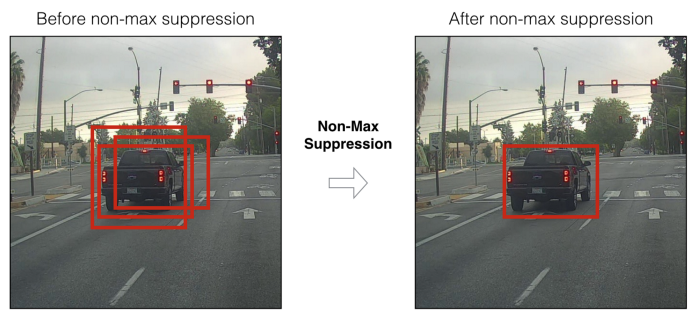
\includegraphics[width=10cm]{imgs/nms_before_after.png}
    \caption{Predicted bounding boxes before and after a non-maximum suppression was applied \cite{nms_before_after}}
    \label{fig:nms_before_after}
\end{center}
\end{figure}

\subsubsection{Regions with CNN Features (R-CNN)}
While the sliding window approach is effective, it is also highly inefficient, since every generated has to be processed in order to find all possible objects in an image.
\ac{R-CNN} by Girshick et al. \cite{rcnn} improves on that by using a region proposal algorithm to obtain probable regions of an object.
In their work the Selective Search algorithm \cite{selective_search} was used to generate region proposals.
Selective Search produces sub-segmentations of objects in an image, considering size, color, texture and shape based features for the grouping of the regions.
How the algorithm performs and what kind of bounding boxes are produced, can be seen in fig. \ref{fig:selective_search}, where the size of the regions is increased from left to right.
The second row of the fig. additionally shows the proposed bounding boxes.
$2000$ of those proposed bounding boxes are taken from different scales and warped into the input shape of the following \ac{CNN}, disregarding the size or aspect ratio of the proposed bounding box.
Each of the bounding boxes is separately passed through the \ac{CNN} and yields a $4096$-dimensional feature vector.
In the next step the $4096$-dimensional feature vector is fed into $N + 1$ binary \acp{SVM}, where $N$ is the number of classes to predict plus one background class.
To further improve the bounding box additionally a bounding box regressor is trained for each class as describe in \cite{bbox_regressor}.

\begin{figure}
\begin{center}
    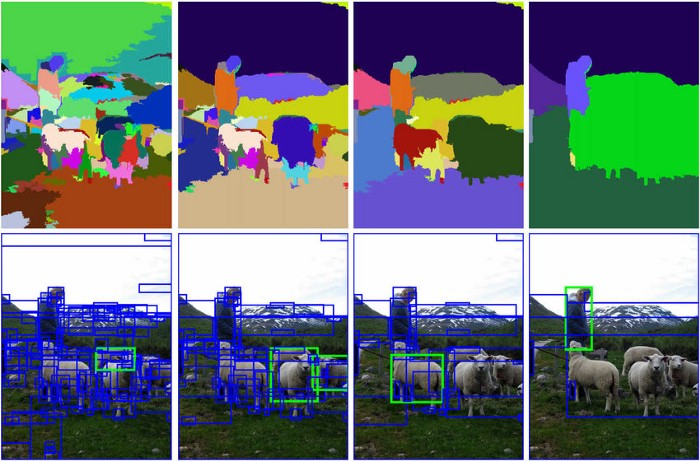
\includegraphics[width=10cm]{imgs/selective_search.png}
    \caption{Example of results obtained through the Selective Search algorithm with increasing region scale from left to right \cite{selective_search}}
    \label{fig:selective_search}
\end{center}
\end{figure}

\subsubsection{Fast R-CNN}
While \ac{R-CNN} was an improvement to the previous methods, the training and inference process was still very expensive, since it involved multiple stages.
First a \ac{CNN} had to be fine tuned. One \ac{SVM} had to be trained for each existing class, which involved saving a lot of \ac{CNN} produced features to a hard drive.
Lastly a bounding box regressor for each class had to be trained.
Furthermore, the inference process took around $47$s per image with a VGG16 \cite{vgg} backbone. \cite{fast_rcnn}

With his work on Fast R-CNN Girshick \cite{fast_rcnn} improved on the training and inference time by a large margin in contrast to \ac{R-CNN}.
He was able to perform the training process with a VGG16 network $9$ times faster and the inference $213$ times faster.

The main difference to \ac{R-CNN} is that instead of generating region proposals, warping them to the input size of the \ac{CNN} and passing them through the \ac{CNN}, region proposals are now projected onto the feature maps of the \ac{CNN} and pooled into a fixed size grid through a \ac{RoI} pooling layer.
Meaning that now the \ac{CNN} computations are now shared between each bounding box proposal resulting in a drastic inference speed improvement.
After pooling the \ac{RoI} it is processed by a fully-connected layer, producing a so called \ac{RoI} feature vector.
This feature vector is fed into a siblings output layer.
The first branch is a classification layer with a softmax output, producing class probabilities and replaces the previous \acp{SVM}, since it showed to perform on par with the \acp{SVM}.
The second branch is comprised of a bounding box regression layer, which outputs bounding box regression offsets as in \ac{R-CNN} \cite{rcnn}.
Due to the one-stage nature of the pipeline a novel multi-task loss was required,
which the author defined as follows:

\begin{equation}
    L(\hat{y}, y, \hat{b}, b) = L_{cls}(\hat{y}, y) + \lambda L_{loc}(\hat{b}, b)
\end{equation}

$\hat{y}$ being the predicted class probabilities by the softmax layer and $y$ the ground truth class.

- TODO should I even do that further?

\subsubsection{Faster R-CNN}
In Fast \ac{R-CNN} the prediction time was decreased by compressing the multi-stage pipeline into a single-stage pipeline.
The remaining non-learnable part of the pipeline became the region proposal algorithm.
It still took around $2s$ to propose bounding boxes with Selective Search.
Ren et. al therefore proposed Faster \ac{R-CNN} \cite{faster_rcnn} to further increase the performance of the overall algorithm.
In Faster \ac{R-CNN} the performance is boosted through the novel \ac{RPN}.
As with Fast \ac{R-CNN} an image is first fed to the \ac{CNN} to produce feature maps.
Afterwards, the feature maps are used as an input to the \ac{RPN}.
The \ac{RPN} operates in a sliding window fashion, where a window size of $nxn$ ($n = 3$) is used to traverse the whole feature map and produce features for the following network.

\begin{figure}
\begin{center}
    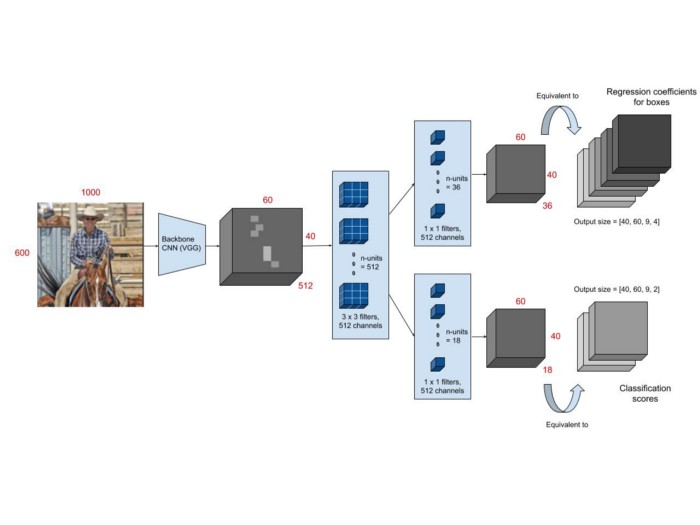
\includegraphics[width=14cm]{imgs/faster_rcnn.jpg}
    \caption{The Faster R-CNN Network Architecture \cite{faster_rcnn_pic} TODO img quality sucks}
    \label{fig:faster_rcnn}
\end{center}
\end{figure}

\subsubsection{Single Shot Detector}

\subsubsection{TODO? Anchor Box Free Detection?}


\subsection{Intersection Over Union (IoU)}

The \ac{IoU}, which is also known as the Jaccard index, is a measure for how much two arbitrary shapes (volumes) are overlapping \cite{giou}.
In object detection \ac{IoU} is often used to compare two bounding boxes and also to construct various loss functions as well as metrics. TODO a bit more; maybe also cite last sentence; last sentence sucks

\begin{equation}
    IoU(A, B) = \frac{|A \cap B|}{|A \cup B|} = \frac{| A \cap B |}{|A| + |B| - |A \cap B|}
\end{equation}


\subsection{IoU Based Loss Functions}

The \ac{MSE} has shown to perform not well for the task of bounding box regression, because it assumes that each regressed variable ($x$, $y$, $w$, $h$) is independent and can be optimized separately \cite{iou}.

To take the correlation of those variables into account, Yu et al. \cite{iou} proposed the \ac{IoU} Loss (eq. \ref{eq:iou_loss}).
While this was a major improvement to previously known methods the \ac{IoU} Loss still suffers from slow convergence and from the gradient vanishing problem, which occurs when the two bounding boxes $A$ and $B$ have no intersection.

\begin{equation}
    L_{IoU} = 1 - IoU(A, B)
    \label{eq:iou_loss}
\end{equation}

Further, to solve these drawbacks Rezatofighi et al. \cite{giou} proposed the \ac{GIoU} Loss (eq. \ref{eq:giou_loss}).
Their loss introduces an additional penalty term added to the \ac{IoU} Loss.
Here, $C$ is the smallest convex box enclosing $A$ and $B$.
Hence, when the boxes have no overlap there is still a gradient pushing them closer to each other.
While the \ac{GIoU} Loss is a major improvement in terms of vanishing gradient, it suffers from slow convergence when $A$ and $B$ have overlap and at the same time $A$ contains $B$ (or vice versa), because the penalty term then becomes $0$, as a consequence the \ac{GIoU} Loss becomes the \ac{IoU} Loss.
Furthermore, it has been observed that when $A$ and $B$ have no overlap, instead of decreasing the spatial distance between $A$ and $B$, the \ac{GIoU} Loss tends to increase the size of the bounding box area to reduce the loss \cite{eiou}.

\begin{equation}
    L_{GIoU} = 1 - IoU(A, B) + \frac{|C - (A \cup B)|}{|C|}
    \label{eq:giou_loss}
\end{equation}

The next improvement in the \ac{IoU} based loss function space was proposed by Zheng et al. \cite{diou}, with their \ac{DIoU} and \ac{CIoU} Loss functions.
In contrast to \ac{GIoU}, \ac{DIoU} (eq. \ref{eq:diou_loss}) solves the gradient vanishing problem by considering the normalized distance of the central points of the two bounding boxes.
The squared euclidean distance is normalized by the squared diagonal length of the smallest box containing $A$ and $B$.

\begin{equation}
    L_{DIoU} = 1 - IoU(A, B) + \frac{\|(A_{center} - B_{center})\|^2}{\|C_{diag}\|^2}
    \label{eq:diou_loss}
\end{equation}

To further improve on that, the authors additionally considered the aspect ratio of the bounding box to be another important geometric factor for bounding box regression.
Hence, the \ac{DIoU} Loss is further extended by a penalty term considering the aspect ratio and resulting in the improved \ac{CIoU} Loss (eq. \ref{eq:ciou_loss}, \ref{eq:ciou_nu}, \ref{eq:ciou_alpha}).
The penalty in \ac{CIoU} is split into $\alpha$ and $\nu$.
$\alpha$ is a trade-off parameter which gives higher priority to the overlapping factor, especially in the case of non-overlap.
Further, $\nu$ is the parameter penalizing the difference in the aspect ratios of $A$ and $B$.
Still, it can be noticed that the $\nu$ is $0$ when the aspect ratios are the same, regardless of the underlying relations between $A_w$, $B_w$ and $A_h$, $B_h$.
E.g. the aspect ratio is the same for all boxes with the following property $\{ (A_w=kB_w, \ A_h=kB_h)\ |\ k \in \R^+\}$ \cite{eiou}.

\begin{equation}
    L_{CIoU} = DIoU(A, B) + \alpha(A,B) * \nu(A, B)
    \label{eq:ciou_loss}
\end{equation}

\begin{equation}
    \nu(A, B) = \frac{4}{\pi^2} [arctan(\frac{A_w}{A_h}) - arctan(\frac{B_w}{B_h})]^2
    \label{eq:ciou_nu}
\end{equation}

\begin{equation}
    \alpha(A, B) = \frac{\nu}{1 - IoU(A, B) + \nu'}
    \label{eq:ciou_alpha}
\end{equation}

Therefore, Zhang et al. \cite{eiou} proposed the \ac{EIoU} Loss to remove this error.
The aspect ratio penalty is here replaced through two separate penalties, which consider the normalized width and height of the two bounding boxes.

- TODO they also incorporated focal loss into that, maybe say that too, at least when I use it

\begin{equation}
    L_{EIoU} = 1 - IoU(A, B) + \frac{\|(A_{center} - B_{center})\|^2}{\|C_{diag}\|^2} + \frac{\|(A_{w} - B_{w})\|^2}{\|C_w\|^2} + \frac{\|(A_{h} - B_{h})\|^2}{\|C_h\|^2}
    \label{eq:eiou_loss}
\end{equation}

\subsection{Anchor Boxes}

- TODO meh

Various object detection networks such as, Faster \ac{R-CNN} \cite{faster_rcnn}, \ac{YOLO} \cite{yolov1}, \ac{SSD} \cite{ssd} and RetinaNet \cite{focalloss} use anchor boxes to predict the objects in an image.
Anchor boxes are used to assign a ground truth to a prediction of a network, which is then used to apply a loss on the prediction and hence make the network learn.
For example in Faster \ac{R-CNN} the ground truth bounding box is assigned to an anchor when the \ac{IoU} of the bounding box and the anchor box is greater than a certain threshold.
Anchor boxes can be seen as predictors, who over time get better and better of predicting objects of certain size and aspect ratios \cite{yolov1}.
The scale and aspect ratio is often picked by using the k-means clustering algorithm on the dataset, to obtain optimal scales and aspect rations representing the underlying dataset.
The selection of good anchor box sizes can improve the prediction quality \cite{faster_rcnn}.
